\chapter{Preliminares e Defini\c{c}\~{o}es}

\section{Feixes puramente propagantes com simetria azimutal}
Um feixe de Bessel com simetria axial \'e escrito como na Figura (\ref{figz}):



%*******************************************
\begin{figure*}[ht]
\centering
\subfigure[]{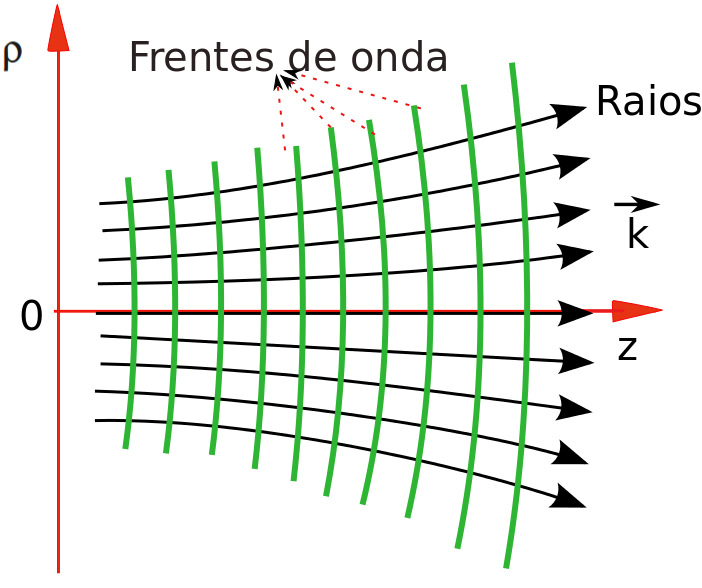
\includegraphics[scale=0.35]{./eps/cap2/roger8.png}}
\subfigure[]{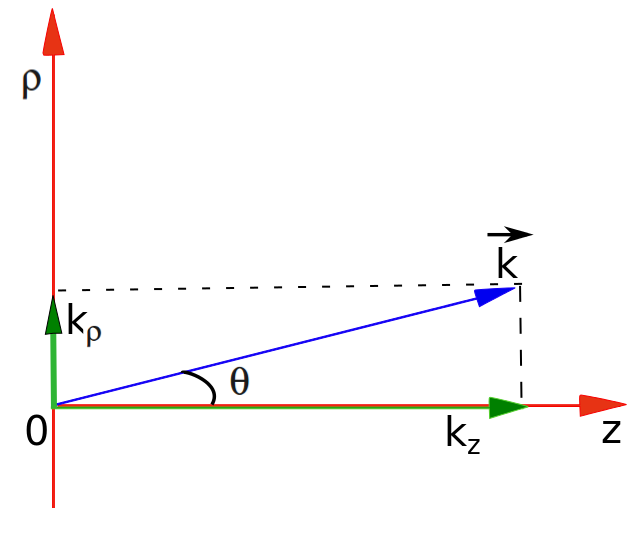
\includegraphics[scale=0.35]{./eps/cap2/roger1.png}}
\caption{(a) Diagrama de raios, onde as normais às frentes de ondas são raios paraxiais. (b-c) Relação entre as componentes do vetor de onda ($k_{\rho}, k_z$). ($b$) Na aproximação paraxial. (c) Fora da aproximação paraxial.}
\label{figz}
\end{figure*}
%********************************************

